% "Станет проще"

\documentclass[a4paper,12pt]{article} % тип документа

% report, book

%  Русский язык

\usepackage[T2A]{fontenc}			% кодировка
\usepackage[utf8]{inputenc}			% кодировка исходного текста
\usepackage{graphicx}
\usepackage[english,russian]{babel}	% локализация и переносы


%отступ

% Математика
\usepackage{amsmath,amsfonts,amssymb,amsthm,mathtools} 
\usepackage{csvsimple}
\usepackage{multirow}


\usepackage{wasysym}
\usepackage{subcaption}
\usepackage{verbatim}
\usepackage{hyperref}
\usepackage{float}
\usepackage{enumerate}
%Заговолок


\begin{titlepage}
\author{Соловьянов Михаил }
\title{Задание 3. Электродинамика. Продвинутые епи постоянного тока и конденсаторы.}
\date{\today}
\end{titlepage}



\begin{document} % начало документа
\maketitle

\begin{figure}[H]
\centering
  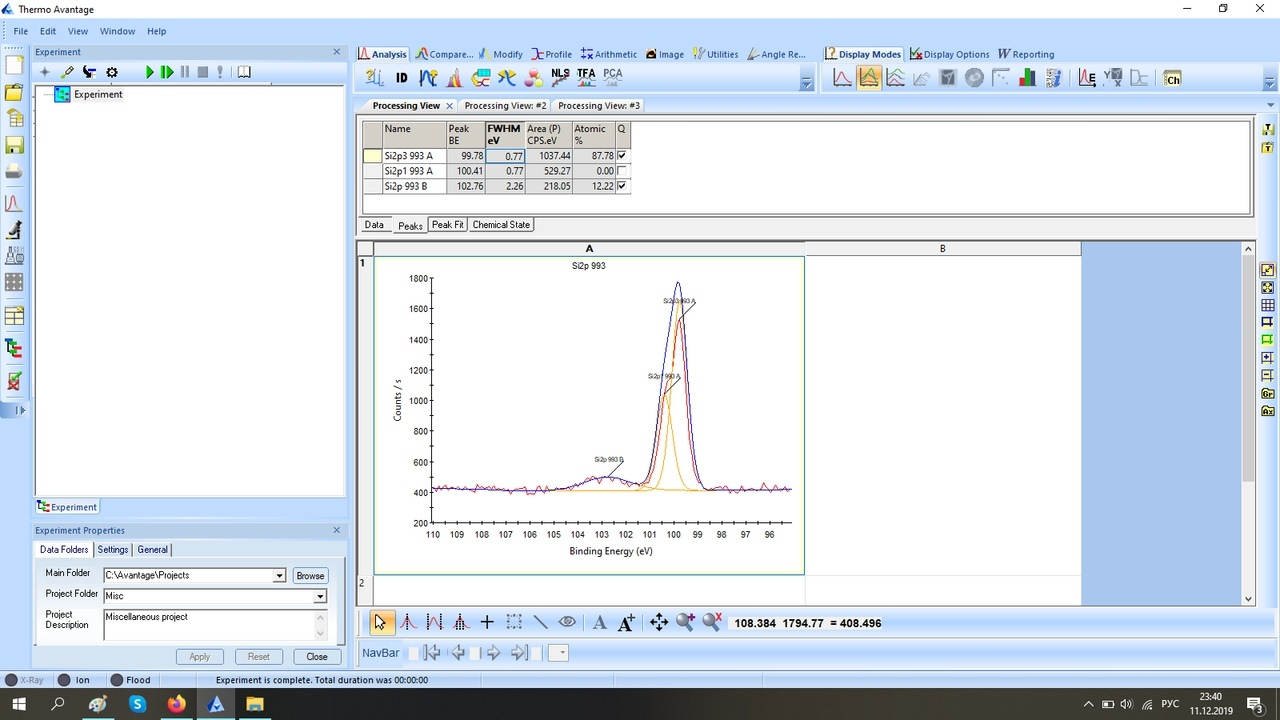
\includegraphics[width=0.5\linewidth]{1.jpg}
  \caption{К задаче 1.}
  \label{fig1}
\end{figure}




\end{document}